%===================================== CHAP 2 =================================

\chapter{Prestudies}

This chapter discusses the research, as well as the decisions made in the pre-development phase of the project. 

\section{Existing solutions}

Following is the evaluation of current existing solutions, that more or less covers the product description. The customer had little to no experience with any of the existing solutions, other than knowledge of their existence, and tasked us to make an evaluation of the applications in question.

\subsection{Apache Apollo}

Apache Apollo\footnote{\url{http://activemq.apache.org/apollo/}} is an open source project maintained by the Apache\footnote{\url{http://www.apache.org}} foundation. This application distinguishes itself from the existing solutions presented below, in the way that it is a complete, protocol agnostic broker, that translates freely between AMQP, MQTT, OpenWire and STOMP. It is an up to date project, that is continually updated by the developer team, and was therefore a very interesting existing solution for us to evaluate.

\subsubsection{Evaluation}

The group set up an instance of Apache Apollo and started reading through both the user and developer documentation. It soon became clear that Apollo is both a very well written broker, and fully or at least partially, covers many of the requirements given by the customer.

The internals of the message queing and message translation systems are very well designed. It uses a non-blocking reactor thread model, which keeps all threads running, and consumes tasks asynchronously, allowing for a vast message processing rate. Another important factor is that Apollo dynamically converts large message queues from actual objects, to pointer references on the fly, when the queue becomes large. This helps mitigate the memory limits of the Java Virtual Machine, and allows Apollo to maintain queues orders of magnitude larger than what a regular in-memory queue system would have.

\subsection{Rabbit MQ}

Rabbit MQ is...

\subsection{WS-Nu}

WS-Nu is a project developed as an assignment at NTNU. It is an implementation of the WSNotification protocol written in Java, thus also an interesting project for us to evaluate.

\section{Software Architecture}

\subsection{Publish-subscribe}

The implementation of the product had to be structured in a publish subscribe messaging pattern. In this pattern, the publishers does not send messages to specific receivers. Instead, messages are placed into categories, and sent to all receivers who subscribes to the category. Publishers and subscribers are seperated, as subscribers do not know which publishers, if any, exists. In the same manner, publishers have no insight into which, if any, subscribers exists to the topic.


\subsection{Architecture draft}

Initial considerations with respect to the overall architecture of the application took place after the first meeting with the customer. The customer put emphasis on a few factors of importance when designing the application. The application protocol implementation had to be modularized in such a way that additional protocol support could be added with ease at a later time. A graphical management interface was also required, to be able to review broker data and adjust publisher/subscriber mappings.

A preliminary draft of a potential application architecture was theorized, which consisted initially of the core broker service, protocol driver modules, publisher and subscriber registry database, management interface, connection handler and message exchange service.

\begin{center}
  \begin{figure}
    \makebox[\textwidth]{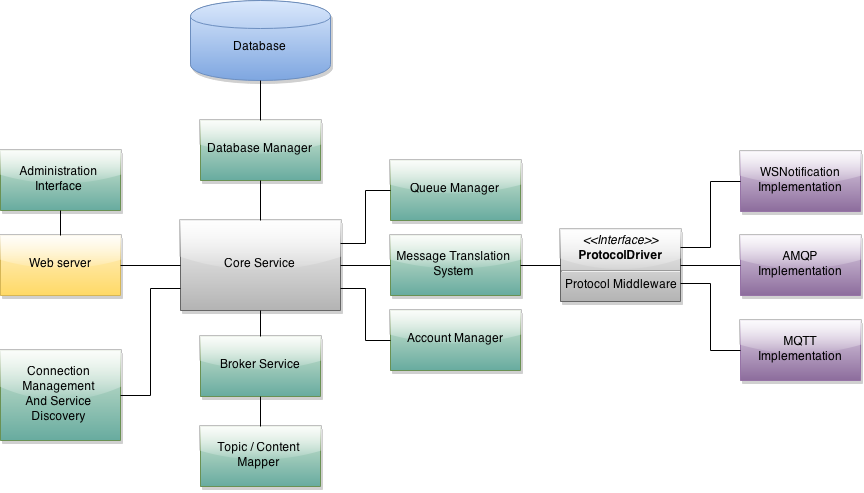
\includegraphics[width=\textwidth]{fig/arch_proposal_aleks.png}}
    \caption{Draft Architecture Proposal}
    \label{fig:arch_proposal}
  \end{figure}
\end{center}

At the same time, evaluation of existing solutions took place, and much interest was given to Apache Apollo\footnote{See section 2.1.1}. Depending on whether we would develop our own, custom tailored broker, or expand on the Apollo project would determine which architecture draft we would develop further. The issue with Apollo however, proved to be the massive code base and previous work done on the implementation. It was clear that the quality of the code, as well as the amount of work put into the product, would be a huge challenge. However, the group chose to commit to the Apollo solution. This was mainly due to the fact that we neither have the knowledge or time to implement a better solution. The proposed custom architecture (fig. \ref{fig:arch_proposal}) was therefore considered to be an alternative solution.

\section{Tools}

\subsection{Skype}

Skype was the main tool used for communication with the customer. Meetings were held using the group call feature of Skype. Communication within the group was done using both group calls, as well as the instant messaging feature within Skype. The tool was convenient to use both for the customer and the group, as well as providing all the communication features needed.

\subsection{Java}

Something something about java version and target SDK.

\subsection{External Java Libraries}

Something something about the external libraries used in this project.

\subsection{JavaDoc}

In this project, the group has chosen to use JavaDoc, an automatic, comment based documentation tool to provide developer documentation of the code base. JavaDoc is supported in most Java Integrated Development Environments (IDE), and allows for easy generation and updating of developer documentation.

\subsection{Intellij IDEA}

Intellij is a Java intergrated development environment(IDE). It contains a wide array of useful functions for development in Java. Such as....

\subsection{Git}

Version control is important when working on a project like this. The group chose to use Git\footnote{\url{http://en.wikipedia.org/wiki/Git_(software)}}, in collaberation with GitHub, a cloud hosted, distributed revision control system that allows all team members to access the code. Git provides complete history and version control, with complete offline support, as the Git working directory acts as a complete repository.

\subsection{Jenkins}

Something something about the automatic setup of the build environment. Dalby, your area.

\subsection{Google Drive}

Google Drive is a platform for sharing documents. Drive supports all nescessary types of files, as well as supporting real time cooperation on documents. In the case of this project, drive is used to share all text and image files used in the report. It also serves as the main platform for sharing time-tables and agendaes for meetings with the customer and supervisor.

\section{Risk analysis}

Following is the risk assessment made early in the planning phase. The diagram shows what was considered to be the most likely events happening, as well as preventive actions. Upon inspection of each of the risks, a number between 1 and 10 was chosen for both the likelyhood of the risk, as well as the potential impact it would have. The final rank of the risk was defined as these two numbers multiplied. 

\begin{center}
  \begin{figure}
    \makebox[\textwidth]{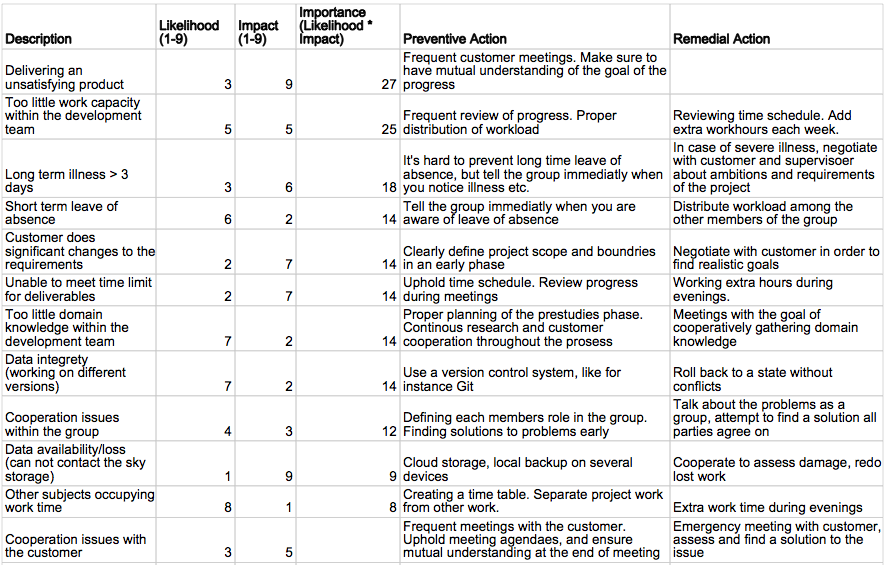
\includegraphics[width=\textwidth]{fig/Riskanalysis.png}}
    \caption{Risk analysis}
    \label{fig:risk_analysis}
  \end{figure}
\end{center}

